\documentclass[11pt]{article}
\usepackage{hyperref}
\usepackage{amsthm}
\usepackage{amsmath}
\usepackage{amsfonts}
\usepackage{tikz}
\usepackage{ wasysym }

\newtheorem{example}{Example}


\author{}
\title{}

\begin{document}
%\maketitle
{\Large
%Change Document name to: Graded Homework 1\_Jacob\_Nicholas
\noindent NAME:  Nicholas Jacob\\ 
STUDENT ID: \# 113578513\\
GRADED HOMEWORK NUMBER: 2\\
COURSE: CS/DSA 4513 DATABASE MANAGEMENT\\ 
SECTION: ONLINE\\SEMESTER: FALL 2023\\
INSTRUCTOR:  DR. LE GRUENWALD\\
 SCORE:}

\newpage
\begin{enumerate}
\item 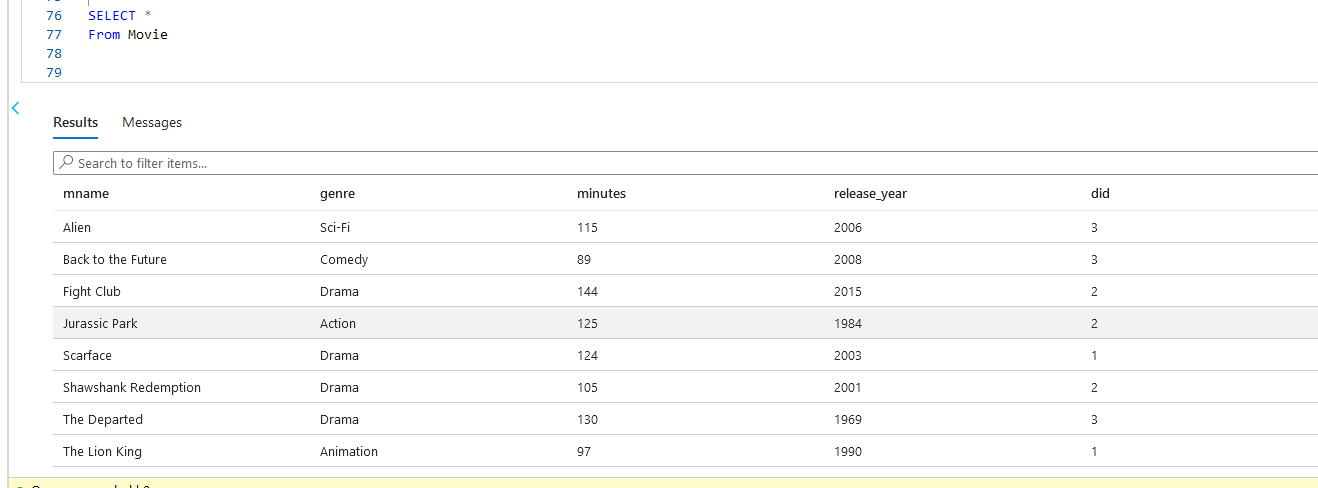
\includegraphics[width = \textwidth]{checktables1.png} 
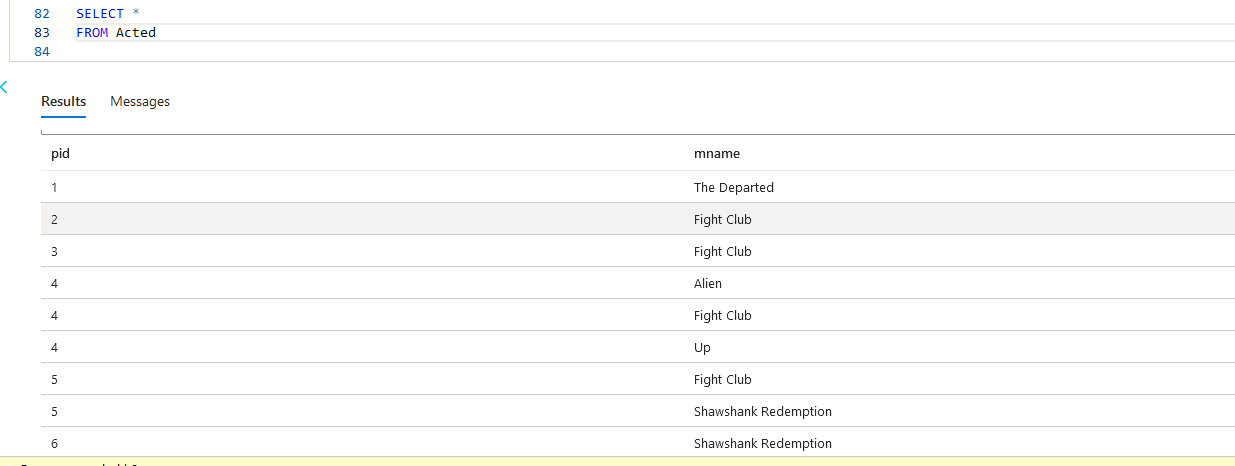
\includegraphics[width = \textwidth]{checktables2.png}
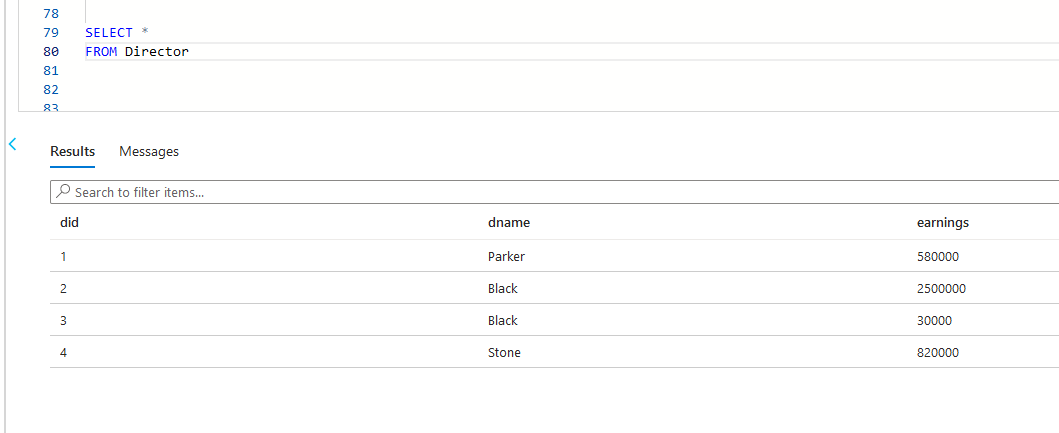
\includegraphics[width = \textwidth]{checktables3.png}
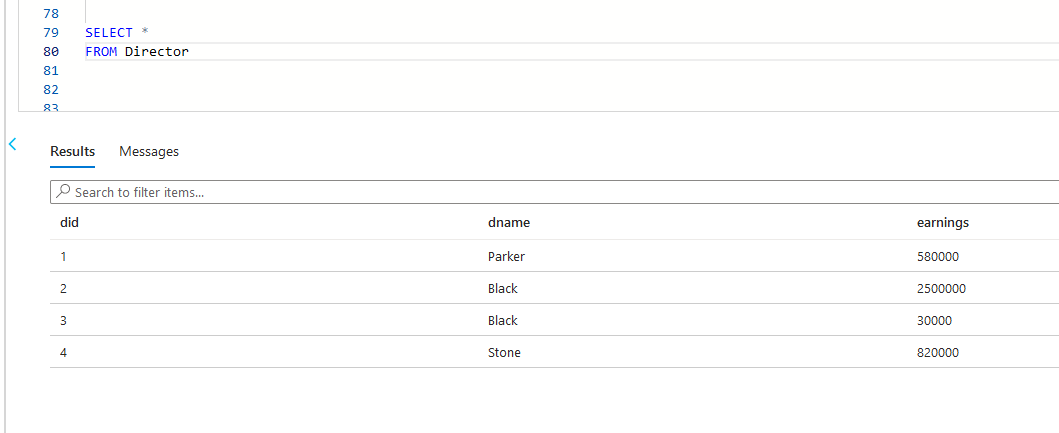
\includegraphics[width = \textwidth]{checktables3.png}
\item 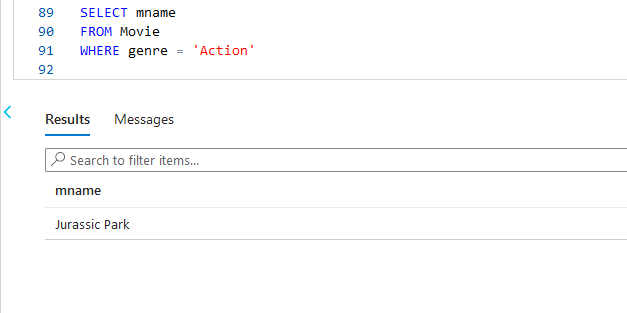
\includegraphics[width = \textwidth]{actionMovies.png}
\item 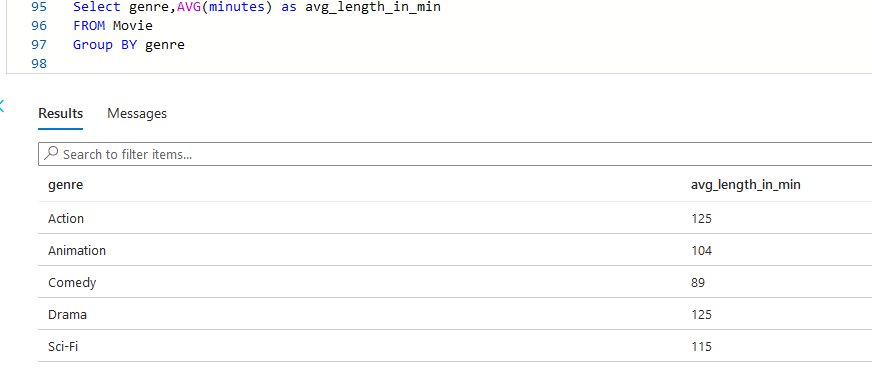
\includegraphics[width = \textwidth]{genreAndLength.png}
\item 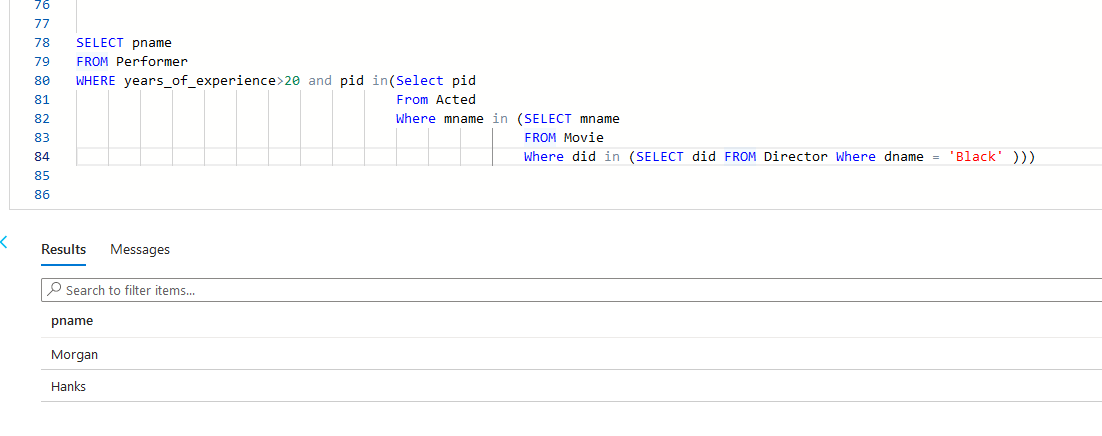
\includegraphics[width = \textwidth]{directedbyblack.png}
\item 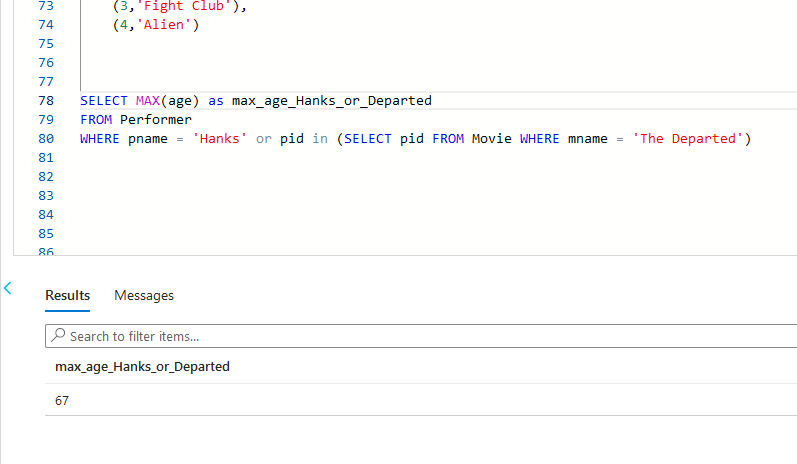
\includegraphics[width = \textwidth]{hanksOrDepartedOldMan.png}
\item 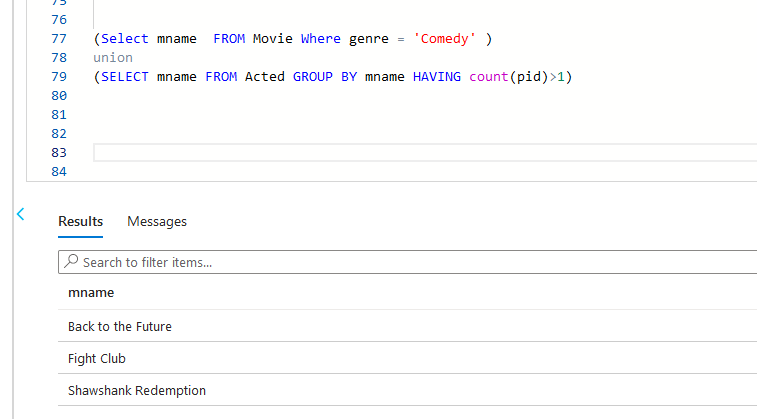
\includegraphics[width = \textwidth]{comedyorLead.png}
\item 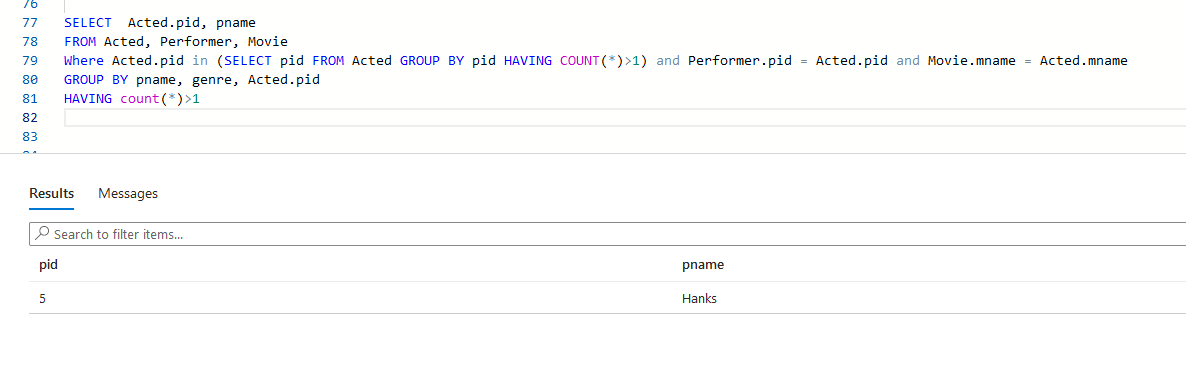
\includegraphics[width = \textwidth]{sameGenre.png}
\item 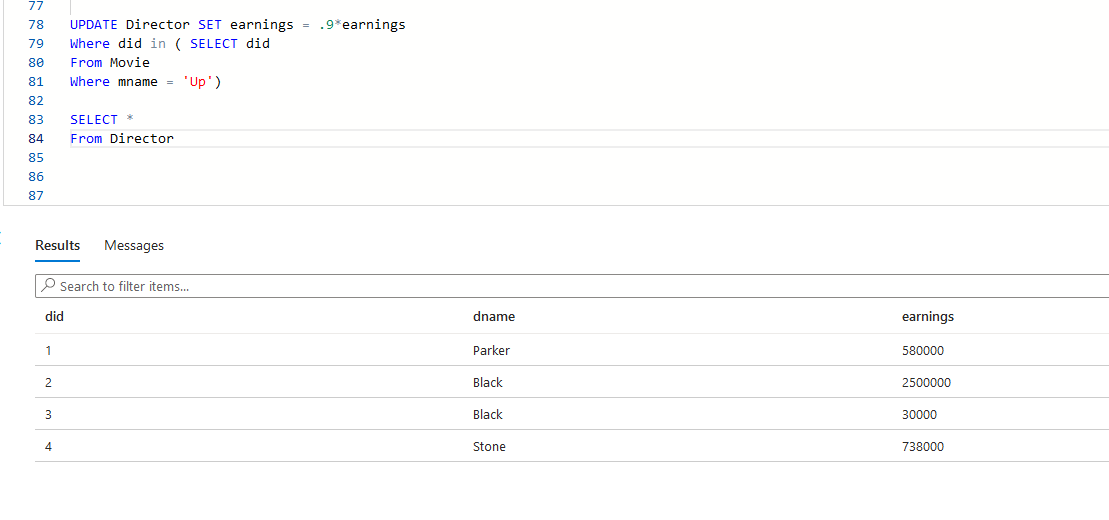
\includegraphics[width = \textwidth]{change.png}
\item 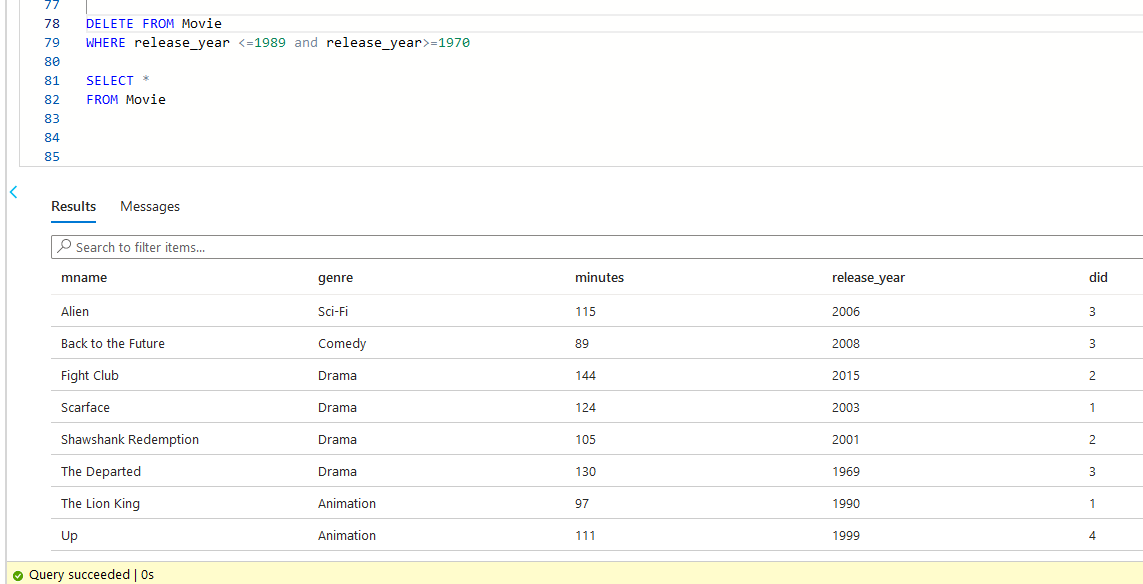
\includegraphics[width = \textwidth]{delete.png}
\end{enumerate}






\end{document}